\subsubsection{Каким образом у УПТ можно обеспечить высокое входное сопротивление?}

Усилителями постоянного тока называют такие устройства, которые могут усиливать медленно изменяющиеся электрические сигналы. Они способны усиливать и переменные и постоянные составляющие входного сигнала. Усилители постоянного тока имеют много разновидностей. Т.к. такие устройства пропускают наряду с переменной составляющей еще и постоянную, то отдельные каскады должны быть связаны между собой либо непосредственно, либо через резисторы, но не через разделительные конденсаторы или трансформаторы, которые не пропускают постоянную составляющую.

Основной проблемой УПТ является т.н. \textbf{Дрейф нуля} - отклонение напряжения на выходе усилителя от начального(нулевого) значения при отсутствии входного сигнала. Основной причиной этого явления является температурная и временная нестабильность активных элементов схемы усилителя, резисторов, источников питания.

Одним из возможных путей уменьшения дрейфа нуля является использование дифференциальных усилителей.

\begin{center}
	\begin{figure}[h!]
		\center{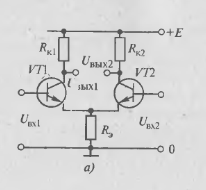
\includegraphics[scale=0.9]{DiffUs.png}}
		\caption{Схема}
	\end{figure}
\end{center} 

Дифференциальный усилительный каскад имеет два входа и усиливает разность напряжений, приложенных к ним. Если на оба входа подать одинаковое(синфазное) напряжение, то усиление будет чрезвычайно мало. Т.о., дифкаскад не усиливает синфазный сигнал. Дифференциальный каскад состоит из двух транзисторов, эмиттеры которых соединены и подключены к общему резистору $R_e$. Для сигнала $U_{in_1}$ транзистор VT1 включен по схеме с ОЭ, VT2 - с ОБ. Для второго сигнала симметрично.

Т.к. дифкаскад часто используется в связке с другими, более сложными каскадами(или является их частью), нужно обеспечить, чтобы на вход ему подавался достаточный сигнал.

Входное сопротивление для разностного сигнала(парафазного, дифференциального) определяется следующим образом:
$$
R_{in} = \frac{\Delta U_{in}}{I_{in}} = 2R_{inTR_{oe}}
$$

видно, что входное сопротивление невелико. В целях повышения его можно включить в цепь эмиттера каждого из транзисторов раные по значению сопротивления резисторы $R_0$ так, чтобы $r_{e_{dif}}$ стало равным $r_{e_{dif}} + R_0$. Однако нельзя ставить слишком большие резисторы, т.к. можно нарушить режим работы усилителя.

Можно снижать коллекторные токи, что ведёт к увеличению $r_{e_{dif}}$, но тогда жертвуем коэффициентом усиления.
\pagebreak

Можно выполнить ДУ на составных транзисторах:

\begin{center}
	\begin{figure}[h!]
		\center{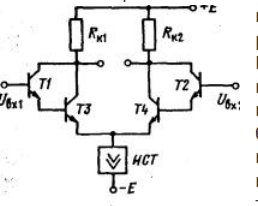
\includegraphics[scale=0.9]{DUs.png}}
		\caption{ДУ на составных транзисторах}
	\end{figure}
\end{center} 

Отметим, что помимо всего прочего, составной транзистор позволит получить больший коэффициент усиления по току. Кроме того, входное сопротивление теперь будет пропорционально $B^2$.





